\documentclass{standalone}

\usepackage{tikz}

\usetikzlibrary{positioning, chains, shapes.geometric, fit, shapes, arrows.meta, calc, backgrounds}

\begin{document}

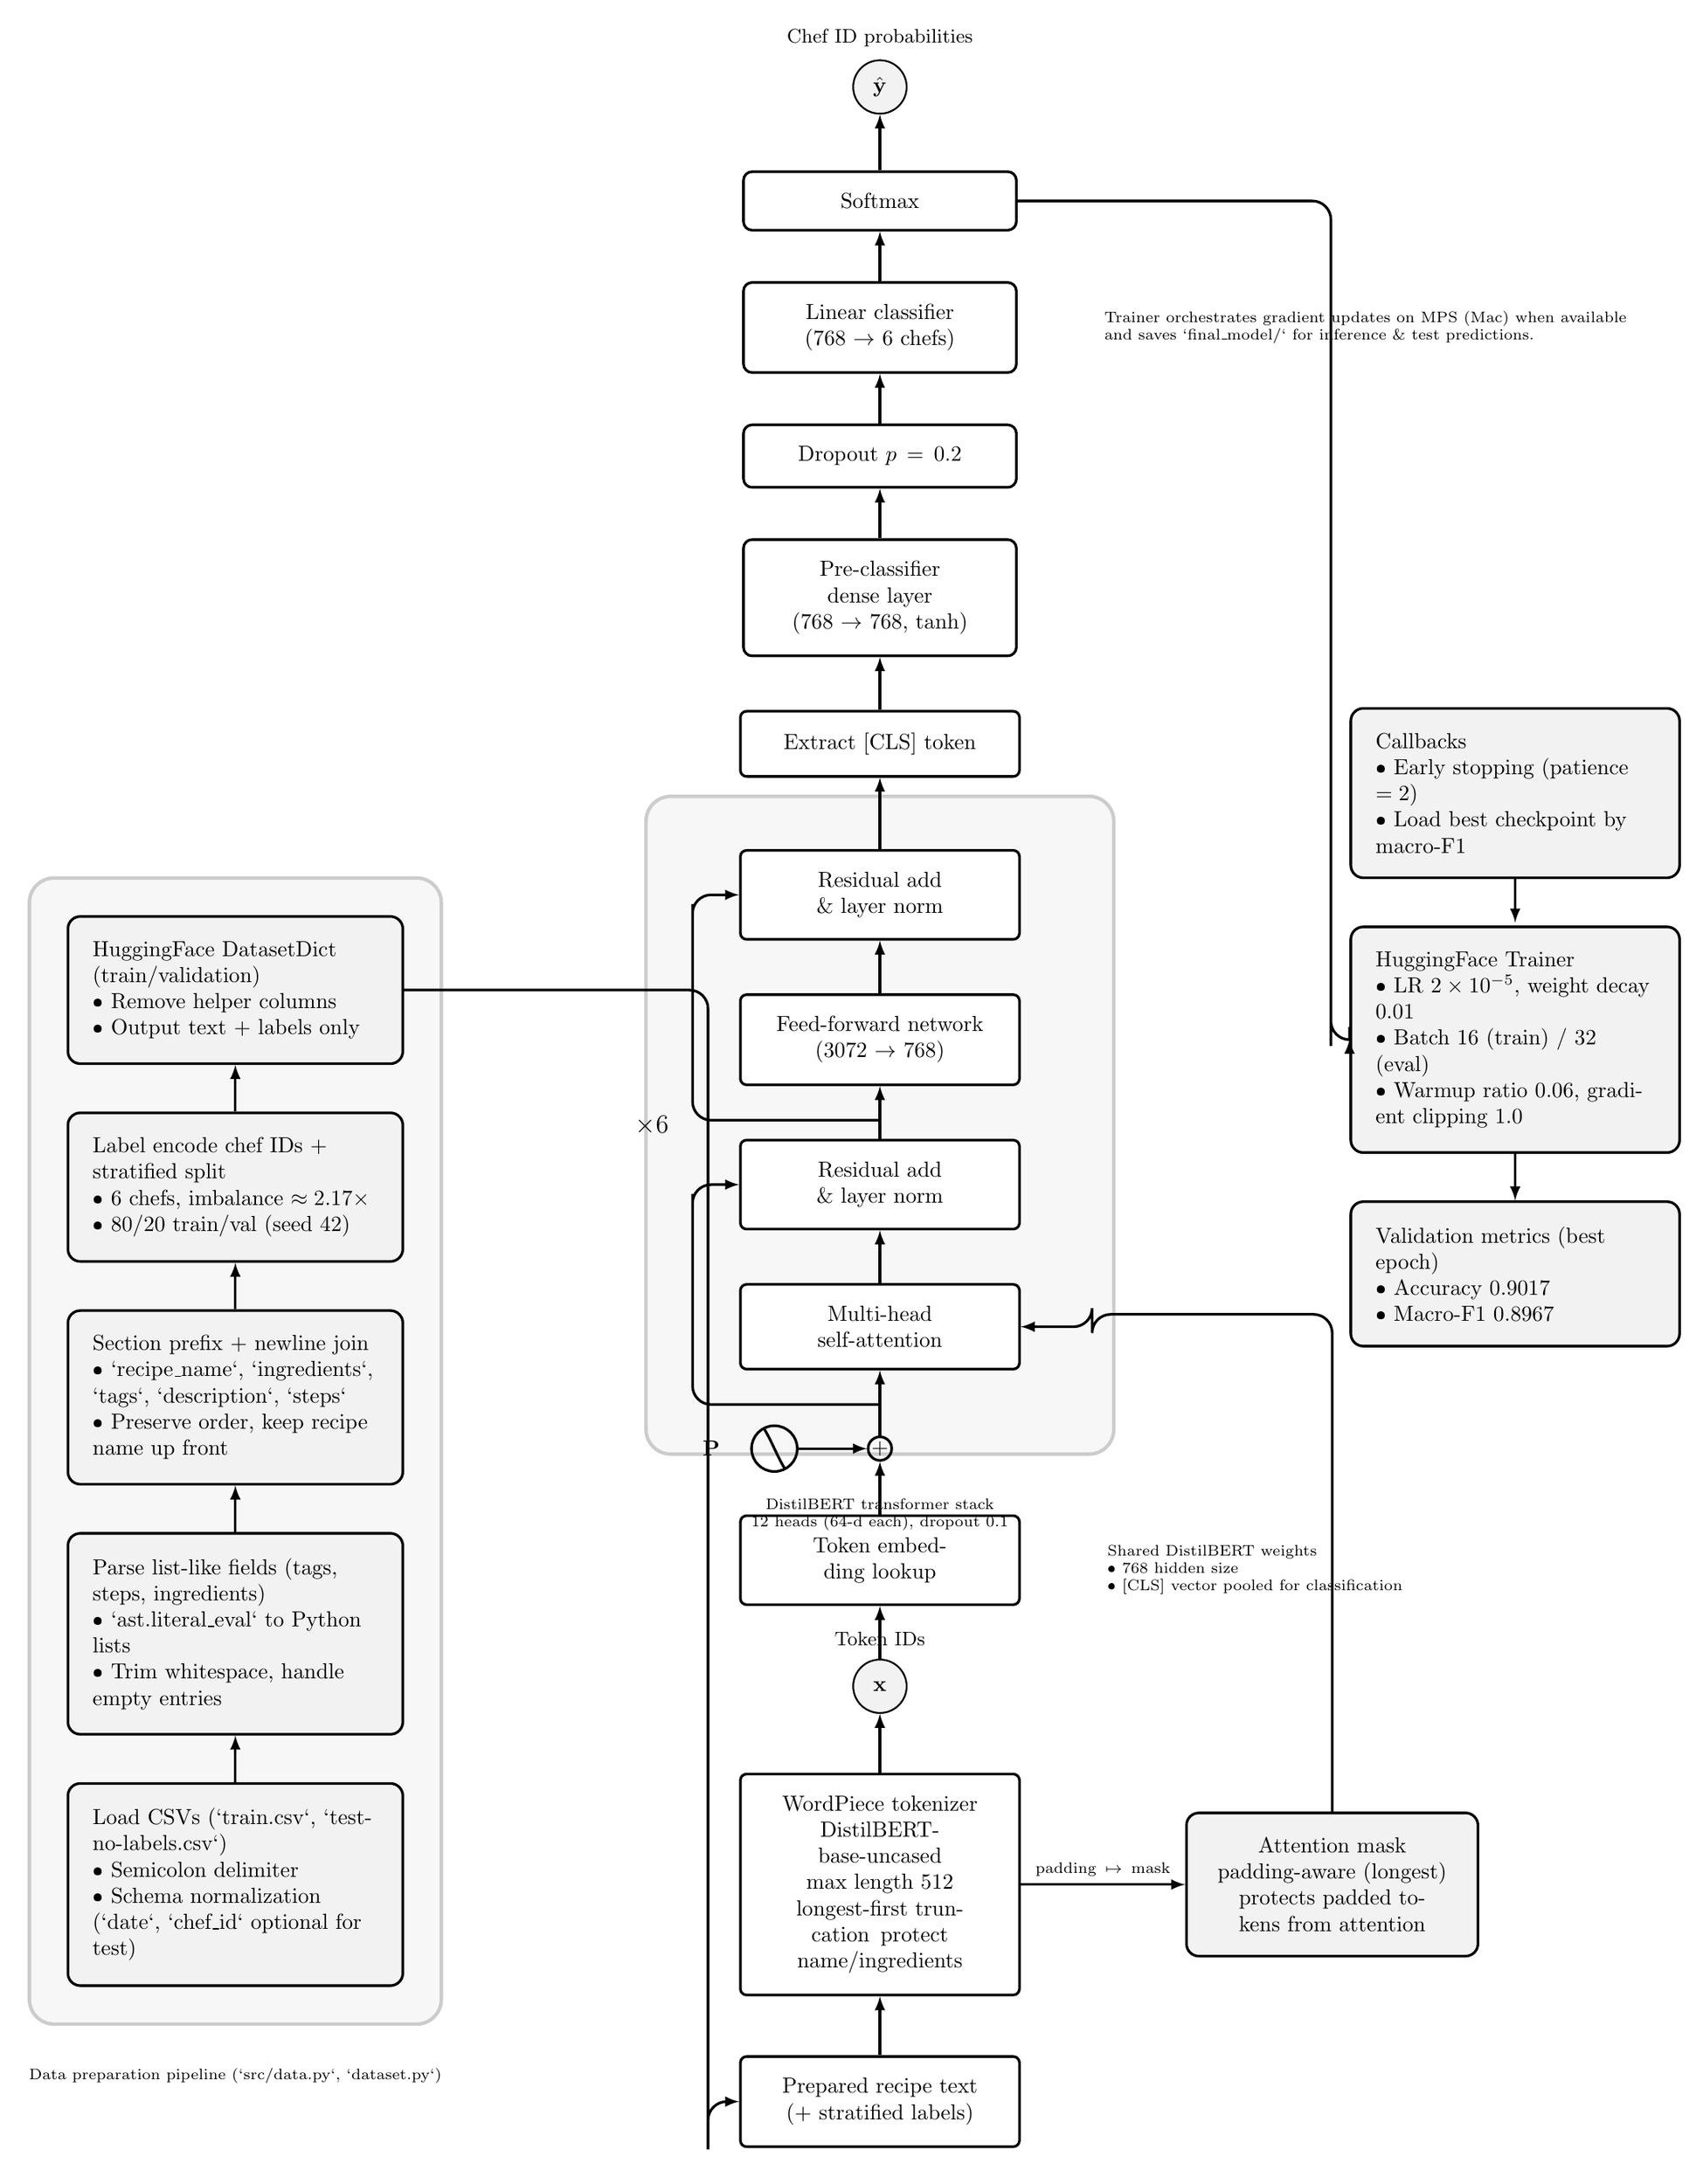
\begin{tikzpicture}[
    >=LaTeX,
    node distance=1.05cm and 2.6cm,
    very thick,
    arrow/.style={
        -latex,
        very thick,
        rounded corners=0.3cm
    },
    process/.style={
        rectangle,
        fill=gray!10,
        rounded corners=2mm,
        draw,
        very thick,
        text width=4.3cm,
        minimum height=1.35cm,
        align=left,
        inner xsep=0.4cm,
        inner ysep=0.4cm
    },
    layer/.style={
        rectangle,
        fill=white,
        rounded corners=1mm,
        inner xsep=0.45cm,
        inner ysep=0.35cm,
        minimum height=1.4em,
        align=center,
        text width=3.6cm,
        draw,
        very thick
    },
    head/.style={
        rectangle,
        fill=white,
        rounded corners=1.4mm,
        inner xsep=0.4cm,
        inner ysep=0.35cm,
        text width=3.6cm,
        align=center,
        draw,
        very thick
    },
    annotation/.style={
        font=\scriptsize,
        align=left
    },
    input/.style={
        circle,
        minimum width=2.45em,
        draw,
        fill=gray!10,
        thick
    },
    capsule/.style={
        rounded corners=4mm,
        draw,
        ultra thick,
        color=gray!40,
        inner sep=0.6cm
    },
    do path picture/.style={%
        path picture={%
          \pgfpointdiff{\pgfpointanchor{path picture bounding box}{south west}}%
            {\pgfpointanchor{path picture bounding box}{north east}}%
          \pgfgetlastxy\x\y%
          	ikzset{x=\x/2,y=\y/2}%
          #1
        }
    },
    sin wave/.style={do path picture={
        \draw [line cap=round] (-3/4,0)
        sin (-3/8,1/2) cos (0,0) sin (3/8,-1/2) cos (3/4,0);
        }
    }
]

    %%%%%%%%%%%%%%%%%%%%%%%%%%%%%%%%%%%%%%%%%%%%%%%%%%%%%%%%%%%%%%
    % Center column: DistilBERT encoder + classifier
    %%%%%%%%%%%%%%%%%%%%%%%%%%%%%%%%%%%%%%%%%%%%%%%%%%%%%%%%%%%%%%
    \node[layer, align=center] (textprep) {Prepared recipe text\\(+ stratified labels)};

    \node[layer, above=0.95cm of textprep, align=center] (tokenizer) {
        WordPiece tokenizer\\DistilBERT-base-uncased\\max length 512\\longest-first truncation\, protect name/ingredients
    };

    \node[input, above=0.95cm of tokenizer] (ids) {$\mathbf{x}$};
    \node[above=0.2em of ids, font=\small] {Token IDs};

    \draw[arrow] (textprep) -- (tokenizer);
    \draw[arrow] (tokenizer) -- (ids);

    \node[layer, above=0.85cm of ids] (tokemb) {Token embedding lookup};
    \draw[arrow] (ids) -- (tokemb);

    \node[circle, draw, minimum size=0.38cm, inner sep=0pt, above=0.85cm of tokemb] (sum1) {$+$};
    \draw[arrow] (tokemb) -- (sum1);

    \node[circle, draw, sin wave, minimum size=2.1em, left=1.1cm of sum1] (pe1) {};
    \node[anchor=east] at ($(pe1.west) + (-0.35,0)$) {$\mathbf{P}$};
    \draw[arrow] (pe1) -- (sum1);

    \node[layer, above=1.05cm of sum1] (attn1) {Multi-head self-attention};
    \node[layer, above=0.85cm of attn1] (add1) {Residual add \& layer norm};
    \node[layer, above=0.85cm of add1] (ff1) {Feed-forward network\\(3072 $\rightarrow$ 768)};
    \node[layer, above=0.85cm of ff1] (add2) {Residual add \& layer norm};

    \draw[arrow] (sum1) -- (attn1);
    \draw[arrow] (attn1) -- (add1);
    \draw[arrow] (add1) -- (ff1);
    \draw[arrow] (ff1) -- (add2);

    \draw[arrow] (attn1.south)++(0,-0.55) -| ($(add1.west) + (-0.75,-0.45)$) |- (add1.west);
    \draw[arrow] (ff1.south)++(0,-0.55) -| ($(add2.west) + (-0.75,-0.45)$) |- (add2.west);

    \coordinate (encSW) at ($(attn1.south west) + (-0.9,-0.75)$);
    \coordinate (encNE) at ($(add2.north east) + (0.9,0.25)$);
    \begin{scope}[on background layer]
        \node[capsule, fill=gray!06] (encoder) [fit=(encSW) (encNE)] {};
    \end{scope}

    \node[anchor=west, font=\large] at ($(encoder.west) + (-0.28,0)$) {$\times 6$};
    \node[annotation, align=center, anchor=north] at ($(encoder.south) + (0,-0.55)$) {
        DistilBERT transformer stack\\12 heads ($64$-d each), dropout $0.1$
    };

    \node[layer, above=1.15cm of add2] (cls) {Extract [CLS] token};
    \node[head, above=0.85cm of cls] (precls) {Pre-classifier dense layer\\(768 $\rightarrow$ 768, tanh)};
    \node[head, above=0.8cm of precls] (dropout) {Dropout $p=0.2$};
    \node[head, above=0.8cm of dropout] (linear) {Linear classifier\\(768 $\rightarrow$ 6 chefs)};
    \node[head, above=0.8cm of linear] (softmax) {Softmax};
    \node[input, above=0.9cm of softmax] (probs) {$\hat{\mathbf{y}}$};
    \node[above=0.2em of probs, font=\small] {Chef ID probabilities};

    \draw[arrow] (add2) -- (cls);
    \draw[arrow] (cls) -- (precls);
    \draw[arrow] (precls) -- (dropout);
    \draw[arrow] (dropout) -- (linear);
    \draw[arrow] (linear) -- (softmax);
    \draw[arrow] (softmax) -- (probs);

    %%%%%%%%%%%%%%%%%%%%%%%%%%%%%%%%%%%%%%%%%%%%%%%%%%%%%%%%%%%%%%
    % Right column: trainer + evaluation context
    %%%%%%%%%%%%%%%%%%%%%%%%%%%%%%%%%%%%%%%%%%%%%%%%%%%%%%%%%%%%%%
    \node[process, right=5.3cm of ff1, text width=4.5cm] (trainer) {
        HuggingFace Trainer\\
        \textbullet\ LR $2\times 10^{-5}$, weight decay $0.01$\\
        \textbullet\ Batch 16 (train) / 32 (eval)\\
        \textbullet\ Warmup ratio $0.06$, gradient clipping 1.0
    };

    \node[process, above=0.75cm of trainer, text width=4.5cm] (callbacks) {
        Callbacks\\
        \textbullet\ Early stopping (patience $=2$)\\
        \textbullet\ Load best checkpoint by macro-F1
    };

    \node[process, below=0.75cm of trainer, text width=4.5cm] (metrics) {
        Validation metrics (best epoch)\\
        \textbullet\ Accuracy $0.9017$\\
        \textbullet\ Macro-F1 $0.8967$
    };

    \node[annotation, align=left, anchor=west] at ($(linear.east) + (1.05,0.0)$) {
        \begin{tabular}{l}
            Trainer orchestrates gradient updates on MPS (Mac) when available\\
            and saves `final\_model/` for inference \& test predictions.
        \end{tabular}
    };

    \draw[arrow] (softmax.east) -| ($(trainer.west) + (-0.3,0.2)$) |- (trainer.west);
    \draw[arrow] (trainer) -- (metrics);
    \draw[arrow] (callbacks) -- ($(trainer.north) + (0,0.05)$);

    %%%%%%%%%%%%%%%%%%%%%%%%%%%%%%%%%%%%%%%%%%%%%%%%%%%%%%%%%%%%%%
    % Left column: data preparation pipeline
    %%%%%%%%%%%%%%%%%%%%%%%%%%%%%%%%%%%%%%%%%%%%%%%%%%%%%%%%%%%%%%
    \node[process, left=5.4cm of tokenizer, text width=4.6cm] (csvload) {
        Load CSVs (`train.csv`, `test-no-labels.csv`)\\
        \textbullet\ Semicolon delimiter\\
        \textbullet\ Schema normalization (`date`, `chef\_id` optional for test)
    };

    \node[process, above=0.75cm of csvload, text width=4.6cm] (parse) {
        Parse list-like fields (tags, steps, ingredients)\\
        \textbullet\ `ast.literal\_eval` to Python lists\\
        \textbullet\ Trim whitespace, handle empty entries
    };

    \node[process, above=0.75cm of parse, text width=4.6cm] (concat) {
        Section prefix + newline join\\
        \textbullet\ `recipe\_name`, `ingredients`, `tags`, `description`, `steps`\\
        \textbullet\ Preserve order, keep recipe name up front
    };

    \node[process, above=0.75cm of concat, text width=4.6cm] (split) {
        Label encode chef IDs + stratified split\\
        \textbullet\ 6 chefs, imbalance $\approx 2.17\times$\\
        \textbullet\ 80/20 train/val (seed 42)
    };

    \node[process, above=0.75cm of split, text width=4.6cm] (dataset) {
        HuggingFace DatasetDict (train/validation)\\
        \textbullet\ Remove helper columns\\
        \textbullet\ Output text + labels only
    };

    \draw[arrow] (csvload) -- (parse);
    \draw[arrow] (parse) -- (concat);
    \draw[arrow] (concat) -- (split);
    \draw[arrow] (split) -- (dataset);
    \draw[arrow] (dataset.east) -| ($(textprep.south west) + (-0.5,-0.2)$) |- (textprep.west);

    \begin{scope}[on background layer]
        \node[capsule, fill=gray!06] (datacapsule) [fit=(csvload) (dataset)] {};
    \end{scope}
    \node[annotation, anchor=north] at ($(datacapsule.south) + (0,-0.55)$) {Data preparation pipeline (`src/data.py`, `dataset.py`)};

    %%%%%%%%%%%%%%%%%%%%%%%%%%%%%%%%%%%%%%%%%%%%%%%%%%%%%%%%%%%%%%
    % Attention mask routing and tokenizer notes
    %%%%%%%%%%%%%%%%%%%%%%%%%%%%%%%%%%%%%%%%%%%%%%%%%%%%%%%%%%%%%%
    \node[process, right=2.65cm of tokenizer, text width=3.9cm, align=center] (mask) {
        Attention mask\\padding-aware (longest)\\protects padded tokens from attention
    };

    \draw[arrow] (tokenizer) -- node[annotation, above, sloped]{padding \,$\mapsto$\, mask} (mask);
    \draw[arrow] (mask.north) |- ($(attn1.east) + (1.15,0.2)$) |- (attn1.east);

    \node[annotation, anchor=west] at ($(tokemb.east) + (1.05,-0.15)$) {
        \begin{tabular}{l}
            Shared DistilBERT weights\\
            \textbullet\ 768 hidden size\\
            \textbullet\ [CLS] vector pooled for classification
        \end{tabular}
    };

\end{tikzpicture}

\end{document}
